\section{Retrieval and Matching Validation}
\label{sec:exp2}

This appendix provides the supporting data for the retrieval and judging claims made in \S\ref{sec:bridging}. We report the judge-calibration study behind our choice of judge of record, bidirectional open-pool retrieval on the blueprint pairs, the cross-project twin candidates surfaced by the same embedding, and the per-bin judging breakdown with representative judged examples.

\subsection{Choosing the judge}\label{app:calib}
Our first judge was Opus~4.8, run on all candidate pairs with a cosine similarity greater than $0.9$; a domain expert then sampled and graded ten of its judged matches. Table~\ref{tab:calib} shows these ten, each with its Opus~4.8 rating, Our expert's verdict and abridged note, and the rating GPT-5.4 produced on the same task. Our expert found Opus to be over-generous on five, over-calling matches as \texttt{exact} where the paper's result was only a special case or a different statement. The over-accepted cases recurred in three ways: the Lean statement was strictly more general than the paper's; a surface match hid a different underlying definition; or a more faithful Lean counterpart existed but was never surfaced.

These slip through because the judge works from compressed evidence. Sloganization abstracts away the hypotheses and definitions that separate a true match from a near one, so the judge over-indexes on the slogan. The Lean signature has the same problem from the other side: a generically named type can carry more specific assumptions than its name suggests, context an author or implementer reads off immediately but the judge never holds.

\begin{table*}[htbp]\centering\small
\begin{tabular}{@{}l c c c c p{6.8cm}@{}}\toprule
formal node & sim & Opus 4.8 & Expert & GPT-5.4 & Expert's note (abridged) \\\midrule
\texttt{append\_assoc} & 0.920 & \bx{green!20}{ex} & \bx{red!22}{wr} & \bx{yellow!35}{inx} & Neither rater grasps the graph structure: Lean's \texttt{SimpleGraph} is loopless (irreflexive), but the paper's graphs allow self-loops. A poor match. \\\addlinespace
\texttt{toMatrix\_adjoint} & 0.968 & \bx{green!20}{ex} & \bx{green!20}{ex} & \bx{yellow!35}{inx} & ``Given bases'' is imprecise from the slogan, but the paper means a unitary isomorphism (orthonormal basis), so it is exact, though not a faithful translation. \\\addlinespace
\texttt{lt\_of\_sub\_pos} & 0.909 & \bx{green!20}{ex} & \bx{green!20}{ex} & \bx{green!20}{ex} & Agree, up to the convention that $\mathbb{N}$ excludes $0$; too trivial to give any insight. \\\addlinespace
\texttt{inner\_tmul} & 0.927 & \bx{green!20}{ex} & \bx{red!22}{wr} & \bx{yellow!35}{inx} & Lean is wrong: Lean's is a general lemma on inner products of tensor products; the paper's is a special family of word spaces, an instance of Lean's theorem at best. \\\addlinespace
\texttt{measureEntropy} & 0.915 & \bx{yellow!35}{inx} & \bx{green!20}{ex} & \bx{yellow!35}{inx} & Outside my area, but Lean's looks slightly more general; likely a strong match. \\\addlinespace
\texttt{norm\_le\_interpStrip} & 0.928 & \bx{green!20}{ex} & \bx{red!22}{wr} & \bx{yellow!35}{inx} & Lean matches the standard Hadamard three-lines theorem, but the paper's printed Lemma~10 reverses the endpoint exponents, so as written it should be judged incorrect. \\\addlinespace
\texttt{iff\_rTensor} & 0.942 & \bx{green!20}{ex} & \bx{yellow!35}{inx} & \bx{yellow!35}{inx} & Exact after specializing to a commutative ring, but the paper's definition is for a left module over a possibly noncommutative ring while Mathlib is commutative-only. Inexact. \\\addlinespace
\texttt{coveringNumber} & 0.926 & \bx{green!20}{ex} & \bx{yellow!35}{inx} & \bx{red!22}{wr} & The informal is the usual \emph{external} covering number; Mathlib's is the \emph{internal} one (covering set $\subseteq A$). \texttt{externalCoveringNumber} is the better match. Inexact at best. \\\addlinespace
\texttt{exists\_prime} & 0.955 & \bx{green!20}{ex} & \bx{green!20}{ex} & \bx{green!20}{ex} & Agree, both are the natural-number form of Bertrand's postulate. An easy one. \\\addlinespace
\texttt{wnorm\_mono} & 0.945 & \bx{green!20}{ex} & \bx{green!20}{ex} & \bx{yellow!35}{inx} & Agree, monotonicity of the weak $L^p$ norm under a.e.\ domination; Lean is more general but a strong match. \\
\bottomrule
\end{tabular}
\caption{Expert calibration of ten Opus~4.8 matches at $\geq\!0.9$. For each candidate: its similarity and the verdicts of the original judge (Opus~4.8), the expert, and the judge of record (GPT-5.4), with the expert's abridged note. \bx{green!20}{ex}=exact, \bx{yellow!35}{inx}=inexact, \bx{red!22}{wr}=wrong. Opus matches the expert on four, over-calls \texttt{exact} on five, and is over-strict on one (\texttt{measureEntropy}); GPT-5.4 is stricter than Opus but, at this sample size, does not fully track the expert.}
\label{tab:calib}
\end{table*}

\subsection{Calibrating the judge of record}\label{app:calib-gpt}
Having rejected Opus, we now validate the judge of record. The same domain expert graded a fresh ten candidates spanning the full $\geq\!0.8$ band, with GPT-5.4's verdict visible only after the expert's own call. Table~\ref{tab:calib-gpt} shows the result.

\begin{table*}[htbp]\centering\small
\begin{tabular}{@{}l c c c p{6.8cm}@{}}\toprule
formal node & sim & Expert & GPT-5.4 & Expert's note (abridged) \\\midrule
\texttt{rpow\_add\_le\_mul\_rpow\_add\_rpow} & 0.974 & \bx{green!20}{ex} & \bx{green!20}{ex} & Same inequality. Lean's \texttt{NNReal} is $[0,\infty)$, potentially slightly stronger than the paper if its $\mathbb{R}_+$ is open. \\\addlinespace
\texttt{PerfectlyNormalSpace} & 0.957 & \bx{green!20}{ex} & \bx{green!20}{ex} & Same definition. The paper's standing ``all spaces are T1'' assumption is slightly stronger than Mathlib's \texttt{PerfectlyNormalSpace}; T1 is bundled separately in \texttt{T6Space}. \\\addlinespace
\texttt{LieSubalgebra.lie\_mem} & 0.927 & \bx{yellow!35}{inx} & \bx{yellow!35}{inx} & Lean is a field accessor on an existing \texttt{LieSubalgebra}; the informal asserts the definition plus the inheritance claim that $\mathfrak{h}$ is itself a Lie algebra. \\\addlinespace
\texttt{alternatingGroup\_le\_\ldots\_isThreeCycle\_mem} & 0.917 & \bx{green!20}{ex} & \bx{green!20}{ex} & Jordan's theorem in both. \texttt{IsPreprimitive} differs from classical primitivity only in nonemptiness, forced here by the 3-cycle; faithfulness is automatic from $G \le \mathrm{Equiv.Perm}\,\alpha$. \\\addlinespace
\texttt{AEMeasurable.lintegral\_prod\_right'} & 0.914 & \bx{red!22}{wr} & \bx{red!22}{wr} & Lean is a.e.-measurability of the inner lower integral on $\mathbb{R}_{\ge 0}^\infty$; informal is the full vector-valued Bochner Fubini theorem. \\\addlinespace
\texttt{Measure.finiteAt\_nhdsWithin} & 0.882 & \bx{red!22}{wr} & \bx{yellow!35}{inx} & Informal is the \emph{definition} of locally finite. Lean is a one-line filter-level consequence assuming it; the faithful counterpart is the class \texttt{IsLocallyFiniteMeasure}. \\\addlinespace
\texttt{HasDerivAt.inner} & 0.880 & \bx{yellow!35}{inx} & \bx{yellow!35}{inx} & Special case of the informal directional-derivative product rule, restricted to ordinary derivatives on $\mathbb{R} \to E$. \\\addlinespace
\texttt{starIsoTerminal\_inv} & 0.865 & \bx{red!22}{wr} & \bx{red!22}{wr} & Informal is the definition of a terminal object. Lean is an equality between two specific morphisms inside the constructed category \texttt{WithTerminal\,C}; uses terminal-object machinery without stating the universal property. \\\addlinespace
\texttt{add\_lt\_add\_of\_le\_of\_lt} & 0.844 & \bx{red!22}{wr} & \bx{red!22}{wr} & Paper is non-strict on both sides; Lean takes mixed non-strict/strict and concludes a strict inequality. The closer counterpart is \texttt{add\_le\_add}. \\\addlinespace
\texttt{map\_neighborFinset\_induce} & 0.822 & \bx{yellow!35}{inx} & \bx{red!22}{wr} & Same structural idea but the paper is directed in-neighborhoods in a sub-tournament; Lean is undirected \texttt{SimpleGraph} neighbors. A faithful cross-category analogue, not the same statement. \\
\bottomrule
\end{tabular}
\caption{Calibration of GPT-5.4 against the expert on ten candidates spanning the full $\geq\!0.8$ band. \bx{green!20}{ex}=exact, \bx{yellow!35}{inx}=inexact, \bx{red!22}{wr}=wrong. GPT-5.4 agrees with the expert on $8/10$ verdicts strictly, and on $9/10$ when collapsed to match/non-match (\texttt{exact}${+}$\texttt{inexact} vs.\ \texttt{wrong}).}
\label{tab:calib-gpt}
\end{table*}

The two disagreements are scope-direction errors in opposite directions. On \texttt{Measure.finiteAt\_nhdsWithin}, the informal is the definition of local finiteness and the Lean lemma is a one-line consequence assuming it; the expert reads this as a level mismatch and grades \texttt{wrong}, GPT-5.4 softens to \texttt{inexact}. On \texttt{map\_neighborFinset\_induce}, the Lean lemma is the same structural statement as the paper's claim transposed from directed graphs to undirected; the expert reads this as a faithful cross-category analogue and grades \texttt{inexact}, GPT-5.4 hardens to \texttt{wrong}.

On the eight agreed verdicts, the expert's and judge's rationales tend to name the same distinction in different words. At the strict-vs-non-strict level (\texttt{add\_lt\_add\_of\_le\_of\_lt}) and at the integration-theory level (\texttt{lintegral\_prod\_right'}) GPT-5.4 catches the gap without prompting. We therefore retain GPT-5.4 as the judge of record, and read the per-bin totals in Table~\ref{tab:judge-breakdown} with the understanding that the strict \texttt{wrong}/\texttt{inexact} split is judge-dependent in the way this calibration documents.


\subsection{Open-pool retrieval}
We also validated retrieval bidirectionally on the blueprint pairs.\footnote{Blueprint pairs are the reference standard throughout this appendix. Confidence intervals on the retrieval and twin-count numbers are $2{,}000$-resample bootstraps (seed~42).} We queried each pair's endpoint and checked whether its annotated partner was returned at rank~1 (Table~\ref{tab:bp-retrieval}). The two directions search different candidate sets. In the formal-to-informal direction ($f\to i$), the formal statement queries the full 11.7M-statement informal corpus, exactly as in the discovery sweep of \S\ref{sec:bridging}. In the informal-to-formal direction ($i\to f$), the informal statement queries only the $36{,}708$ declarations from the formalization projects, not the full \nSwept-declaration formal graph searched in \S\ref{sec:bridging}. This restriction is appropriate because every blueprint \texttt{\textbackslash lean\{\}} target is a project declaration; the remaining Mathlib and Lean-core declarations contain no possible answer and would only add distractors.

We find that disjoint pairs are largely missed across both directions of querying. In particular, $61.2\%$ $[58.9, 63.6]$ of blueprint pairs are recovered by at least one direction, and $22.3\%$ $[20.2, 24.4]$ are mutual rank-1. As a non-semantic baseline, we also reran $i\to f$ over the same project declarations using BM25, a standard lexical ranker based solely on weighted query--candidate term overlap. Because the embedding-based method outperforms BM25 at every cutoff, its matches cannot be explained solely by shared surface vocabulary and instead reflect semantic agreement.

\begin{table}[htbp]
  \centering \small \setlength{\tabcolsep}{5pt}
  \begin{tabular}{lrrrr}
    \toprule
    Sweep & Hit@1 & Hit@5 & Hit@10 & MRR \\
    \midrule
    Embedding $f\to i$  & \textbf{43.5} & 64.8 & 69.9 & 52.5 \\
    Embedding $i\to f$  & \textbf{42.6} & 67.0 & 71.7 & 53.1 \\
    BM25 $i\to f$       & 31.3          & 53.7 & 61.0 & 41.0 \\
    \bottomrule
  \end{tabular}
  \caption{Open-pool retrieval (\%). $n$ is the number of distinct evaluable queries: $1{,}530$ of the $1{,}577$ blueprint formals for $f\to i$ (47 lack an evaluable open-pool partner), $1{,}308$ blueprint informals for $i\to f$. BM25 is a lexical baseline.}
  \label{tab:bp-retrieval}
\end{table}

\subsection{Match types}
Because both graphs are embedded in one space, the same slogan retrieval surfaces three kinds of match depending on which corpora the query and its neighbor come from (Figure~\ref{fig:match-types}): a \emph{formal--informal match} ($f\!\leftrightarrow\!i$), the matches of \S\ref{sec:bridging} which the open-pool retrieval above validates; a \emph{cross-project twin} ($f\!\leftrightarrow\!f$), the same result formalized in two projects, which we probe below; and a \emph{cross-paper restatement} ($i\!\leftrightarrow\!i$), the same result stated in two papers, which we do not pursue here.
\begin{figure}[htbp]
  \centering
  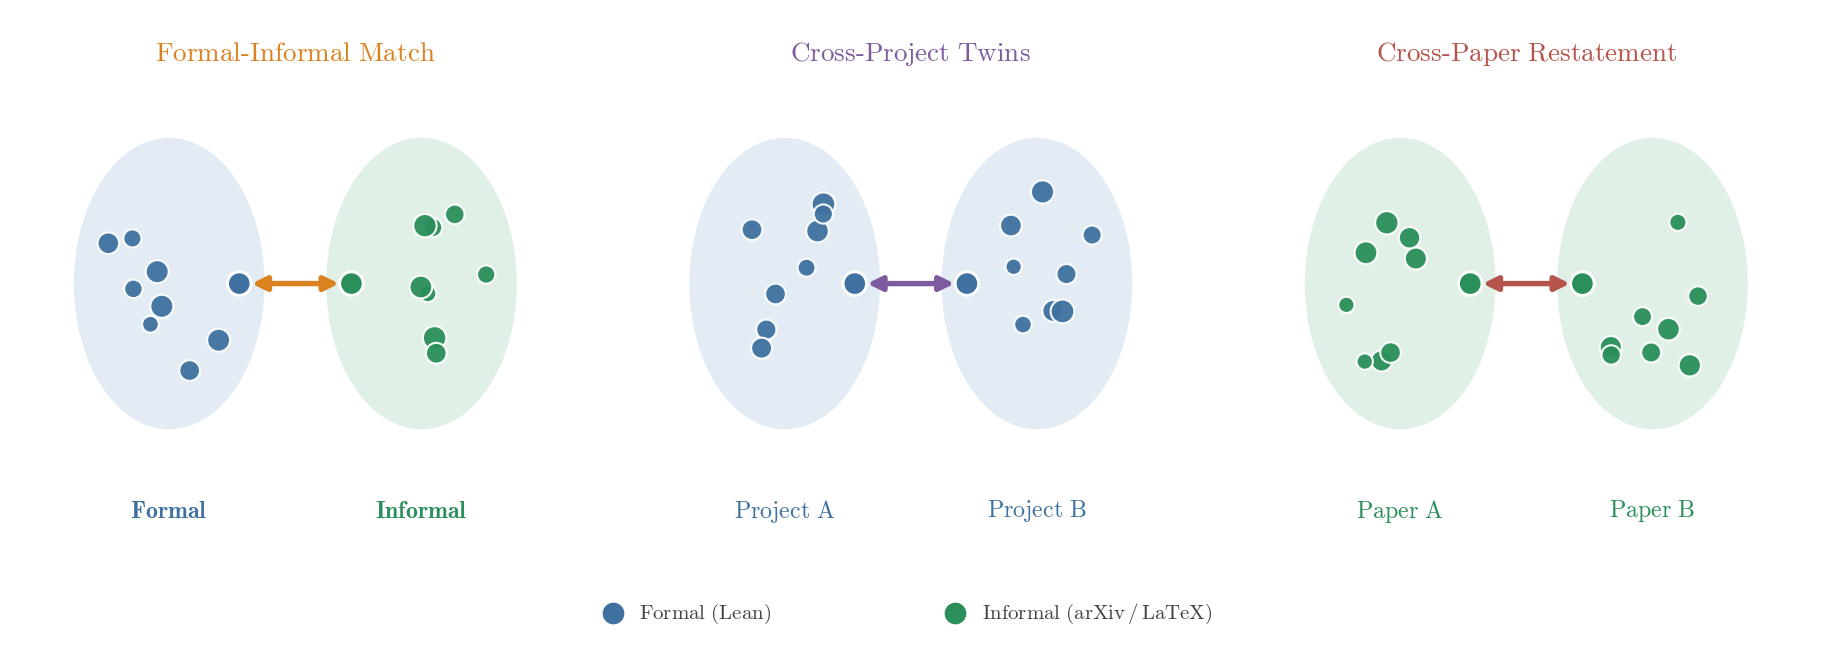
\includegraphics[width=\linewidth]{match_types.png}
  \caption{Three kinds of match the slogan embedding can surface, by the corpora of the query and its nearest neighbor: a formal--informal match ($f\!\leftrightarrow\!i$), a cross-project twin ($f\!\leftrightarrow\!f$), and a cross-paper restatement ($i\!\leftrightarrow\!i$).}
  \label{fig:match-types}
\end{figure}

\subsection{Candidate cross-project twins ($f\to f$)}
The same slogan embedding can be swept formal-to-formal across the project declarations to surface \emph{candidate} twins: a project lemma whose nearest neighbor is a lemma in a different project. Excluding same-paper matches and two parallel-formalization repository pairs, $446$ $[253, 682]$ pairs sit at cosine $\geq 0.85$ (14 at $\geq 0.95$); Table~\ref{tab:twins-examples} lists the highest-cosine ones. Consistent with \S\ref{sec:bridging}, cosine here is a candidate signal, not ground truth: these pairs are \emph{not} judge-confirmed, so the count is a candidate set rather than a verified twin set. Running the same LLM-as-judge step over these candidates to confirm genuine twins is a natural extension we have not yet performed.

\begin{table}[htbp]
  \centering \small \setlength{\tabcolsep}{4pt}
  \begin{tabular}{rp{0.74\linewidth}}
    \toprule
    sim & Candidate twin pair and shared statement \\
    \midrule
    0.999 & \texttt{NNReal.coe\_comp\_dconv} (add-combi) $\leftrightarrow$ \texttt{NNReal.coe\_comp\_cdconv} (apap): the $\mathbb{R}_{\ge 0}\to\mathbb{R}$ coercion commutes with discrete convolution. \\
    \addlinespace
    0.988 & \texttt{$\Phi_4'$\_contDiffOn} (Sphere-Packing-Lean) $\leftrightarrow$ same (sphere-packing-math-inc): $\Phi_4'$ is continuously differentiable on its domain. \\
    \addlinespace
    0.987 & \texttt{neg\_cdconv} (apap) $\leftrightarrow$ \texttt{neg\_conv} (add-combi): negation distributes through the convolution. \\
    \bottomrule
  \end{tabular}
  \caption{Highest-cosine $f\to f$ candidate twins. The top pairs are likely equivalent statements under independent identifier conventions, but the set as a whole is cosine-surfaced and not judge-confirmed.}
  \label{tab:twins-examples}
\end{table}

\subsection{Judging breakdown}
Table~\ref{tab:judge-breakdown} gives the per-bin verdict counts behind Figure~\ref{fig:comp}: for each cosine band, how many judged candidates each model labels \texttt{exact}, \texttt{inexact}, or \texttt{wrong}, and the resulting match rate (\texttt{exact}${+}$\texttt{inexact}). Both judges move from almost all matches at the top of the band, a mix of \texttt{exact} and \texttt{inexact}, to mostly \texttt{wrong} near the floor; DeepSeek is uniformly more generous. The two models judge near-identical candidate sets, with small per-bin differences in $n$ from parse failures and unjudgeable cases.

\begin{table}[htbp]
  \centering \small \setlength{\tabcolsep}{5pt}
  \begin{tabular}{lrrrrr}
    \toprule
    Sim.\ bin & $n$ & \bx{green!20}{exact} & \bx{yellow!35}{inexact} & \bx{red!22}{wrong} & match (\%) \\
    \midrule
    \multicolumn{6}{@{}c}{\itshape GPT-5.4 (judge of record)}\\
    0.95--1.0  &     676 &     290 &     360 &      26 &    650 (96.2) \\
    0.90--0.95 &  6{,}644 & 1{,}391 &  4{,}312 &     941 &  5{,}703 (85.8) \\
    0.85--0.90 & 26{,}755 & 1{,}834 & 14{,}852 & 10{,}069 & 16{,}686 (62.4) \\
    0.80--0.85 & 66{,}537 & 1{,}250 & 23{,}663 & 41{,}624 & 24{,}913 (37.4) \\
    \addlinespace
    \textbf{Total} & 100{,}612 & 4{,}765 & 43{,}187 & 52{,}660 & \textbf{47{,}952 (47.7)} \\
    \midrule
    \multicolumn{6}{@{}c}{\itshape DeepSeek-V4-Pro (lenient comparison)}\\
    0.95--1.0  &     678 &     587 &      80 &      11 &    667 (98.4) \\
    0.90--0.95 &  6{,}645 &  4{,}542 &  1{,}678 &     425 &  6{,}220 (93.6) \\
    0.85--0.90 & 26{,}827 & 11{,}151 &  9{,}195 &  6{,}481 & 20{,}346 (75.8) \\
    0.80--0.85 & 66{,}700 & 14{,}951 & 19{,}050 & 32{,}699 & 34{,}001 (51.0) \\
    \addlinespace
    \textbf{Total} & 100{,}850 & 31{,}231 & 30{,}003 & 39{,}616 & \textbf{61{,}234 (60.7)} \\
    \bottomrule
  \end{tabular}
  \caption{Per-bin judging breakdown for the two judges over the corrected candidate pool ($\geq\!0.8$ cosine), highest band first. Column headers are colored by verdict (\bx{green!20}{exact}, \bx{yellow!35}{inexact}, \bx{red!22}{wrong}); \texttt{exact}${+}$\texttt{inexact} count as matches. GPT-5.4 is our set of record, DeepSeek-V4-Pro a more lenient high-recall comparison; the bold totals contrast the strict (47.7\%) and lenient (60.7\%) overall match rates.}
  \label{tab:judge-breakdown}
\end{table}

\subsection{Judged match examples}
\label{app:matching-examples}
Tables~\ref{tab:matching-verdict} and~\ref{tab:matching-band} show representative GPT-5.4-judged candidate edges from the corrected set, each pairing the formal Lean statement with its informal arXiv counterpart. Table~\ref{tab:matching-verdict} gives one example per verdict class so the difference between a match and a false positive is visible; Table~\ref{tab:matching-band} gives judge-affirmed (\texttt{exact}) matches at a high, mid, and low point of the $0.9$--$1.0$ band.

\begin{table*}[htbp]\centering\small\setlength{\tabcolsep}{6pt}
\begin{tabular}{@{}>{\raggedright\arraybackslash}p{\dimexpr0.5\textwidth-2.8cm\relax} >{\raggedright\arraybackslash}p{\dimexpr0.5\textwidth-2.8cm\relax} >{\footnotesize\raggedright\arraybackslash}p{1.7cm} c c@{}}
\toprule
\textbf{Formal (Lean)} & \textbf{Informal statement} & \multicolumn{1}{l}{\textbf{arXiv}} & sim & verdict \\
\midrule
\lc{niven \{$\theta$ : $\mathbb{R}$\} (h$\theta$ : $\exists$ r, $\theta$ = $\uparrow$r * Real.pi) (hcos : $\exists$ q, Real.cos $\theta$ = $\uparrow$q) : Real.cos $\theta$ $\in$ \{-1, -1 / 2, 0, 1 / 2, 1\}} & Let $\theta$ be a rational multiple of $2\pi$. If $\cos(\theta)\in\mathbb{Q}$, then $\cos(\theta)\in\left\{-1,-\tfrac12,0,\tfrac12,1\right\}$. & 1410.6912 & 0.97 & \bx{green!20}{exact} \\
\addlinespace
\lc{SemidirectProduct.mul\_def \{N : Type u\_1\} \{G : Type u\_2\} [Group N] [Group G] \{$\varphi$ : G $\to$* MulAut N\} (a b : N $\rtimes$[$\varphi$] G) : a * b = $\langle$a.left * ($\varphi$ a.right) b.left, a.right * b.right$\rangle$} & The semidirect product $N\rtimes_\varphi H$ has underlying set $N\times H$ with $(n_1,h_1)(n_2,h_2)=(n_1\varphi(h_1)(n_2),h_1h_2)$. & 2111.00575 & 0.90 & \bx{yellow!35}{inexact} \\
\addlinespace
\lc{Ne.symm \{$\alpha$ : Sort u\} \{a b : $\alpha$\} (h : a $\neq$ b) : b $\neq$ a} & For all $a,b$, if $a=b$ then $b=a$. & 0707.1981 & 0.90 & \bx{red!22}{wrong} \\
\bottomrule
\end{tabular}
\caption{Representative GPT-5.4 verdicts from the corrected candidate set, one per class: the verbatim Lean statement, the paper's informal statement, the arXiv id, the cosine similarity, and the verdict. \texttt{exact}/\texttt{inexact} count as matches; \texttt{wrong} (lexically near but mathematically distinct, e.g.\ \texttt{Ne.symm}: symmetry of $\neq$ vs.\ the paper's $=$) does not.}
\label{tab:matching-verdict}
\end{table*}

\begin{table*}[htbp]\centering\small\setlength{\tabcolsep}{6pt}
\begin{tabular}{@{}>{\raggedright\arraybackslash}p{\dimexpr0.5\textwidth-2.8cm\relax} >{\raggedright\arraybackslash}p{\dimexpr0.5\textwidth-2.8cm\relax} >{\footnotesize\raggedright\arraybackslash}p{1.7cm} c c@{}}
\toprule
\textbf{Formal (Lean)} & \textbf{Informal statement} & \multicolumn{1}{l}{\textbf{arXiv}} & sim & verdict \\
\midrule
\lc{Aux.sum\_inv\_le\_log (n : $\mathbb{N}$) (hn : 1 $\le$ n) : $\sum$ d $\in$ Finset.Icc 1 n, ($\uparrow$d)$^{-1}$ $\le$ 1 + Real.log $\uparrow$n} & For any positive integer $n$, $\sum_{t=1}^{n}\tfrac{1}{t}\le 1+\log n$. & 2002.05359 & 0.98 & \bx{green!20}{exact} \\
\addlinespace
\lc{Real.cos\_sq\_add\_sin\_sq (x : $\mathbb{R}$) : Real.cos x \textasciicircum{} 2 + Real.sin x \textasciicircum{} 2 = 1} & The identity $\sin^2 x+\cos^2 x=1$ holds for $x\in\mathbb{R}$. & 2312.13525 & 0.95 & \bx{green!20}{exact} \\
\addlinespace
\lc{legendreSym.at\_neg\_two \{p : $\mathbb{N}$\} [Fact (Nat.Prime p)] (hp : p $\neq$ 2) : legendreSym p (-2) = ZMod.$\chi_8'$ $\uparrow$p} & If $p$ is an odd prime, $\left(\tfrac{-2}{p}\right)=1$ if $p\equiv 1,3 \pmod 8$ and $-1$ if $p\equiv 5,7 \pmod 8$. & 2309.02512 & 0.91 & \bx{green!20}{exact} \\
\bottomrule
\end{tabular}
\caption{Judge-affirmed (\texttt{exact}) matches from the corrected GPT-5.4 set at a high, mid, and low point of the $0.9$--$1.0$ band (similarity $\approx$ 0.98 / 0.95 / 0.91): the verbatim Lean statement against the paper's informal statement. \texttt{legendreSym.at\_neg\_two} shows the abstract Lean form ($=\chi_8'(p)$) the judge matched to the paper's explicit residue cases.}
\label{tab:matching-band}
\end{table*}